
\chapter{背景介绍}\label{chap:background}
本章介绍相关概念与技术，并梳理 Kubernetes 权限提升漏洞相关的国内外研究现状。

\section{相关概念与技术}

\subsection{容器}

服务应用的部署经历从物理机部署、到虚拟机部署、再到容器化部署的演进过程（见图~\ref{fig:container-evolution}）。虚拟机部署基于KVM等虚拟化技术，实现了完整操作系统模拟与资源隔离与复用，但存在虚拟化开销较大，启动时间较长，镜像体积庞大等问题，影响了应用的交付效率和资源利用率。与传统的物理机和虚拟机相比，容器通过操作系统内核级的资源隔离，实现了更高的资源利用率和更快的启动速度。容器以\textbf{镜像}为交付单元，将部署应用及其依赖环境以镜像形式打包。容器技术原理依赖三类内核技术：
\begin{figure}[htb]
    \centering
    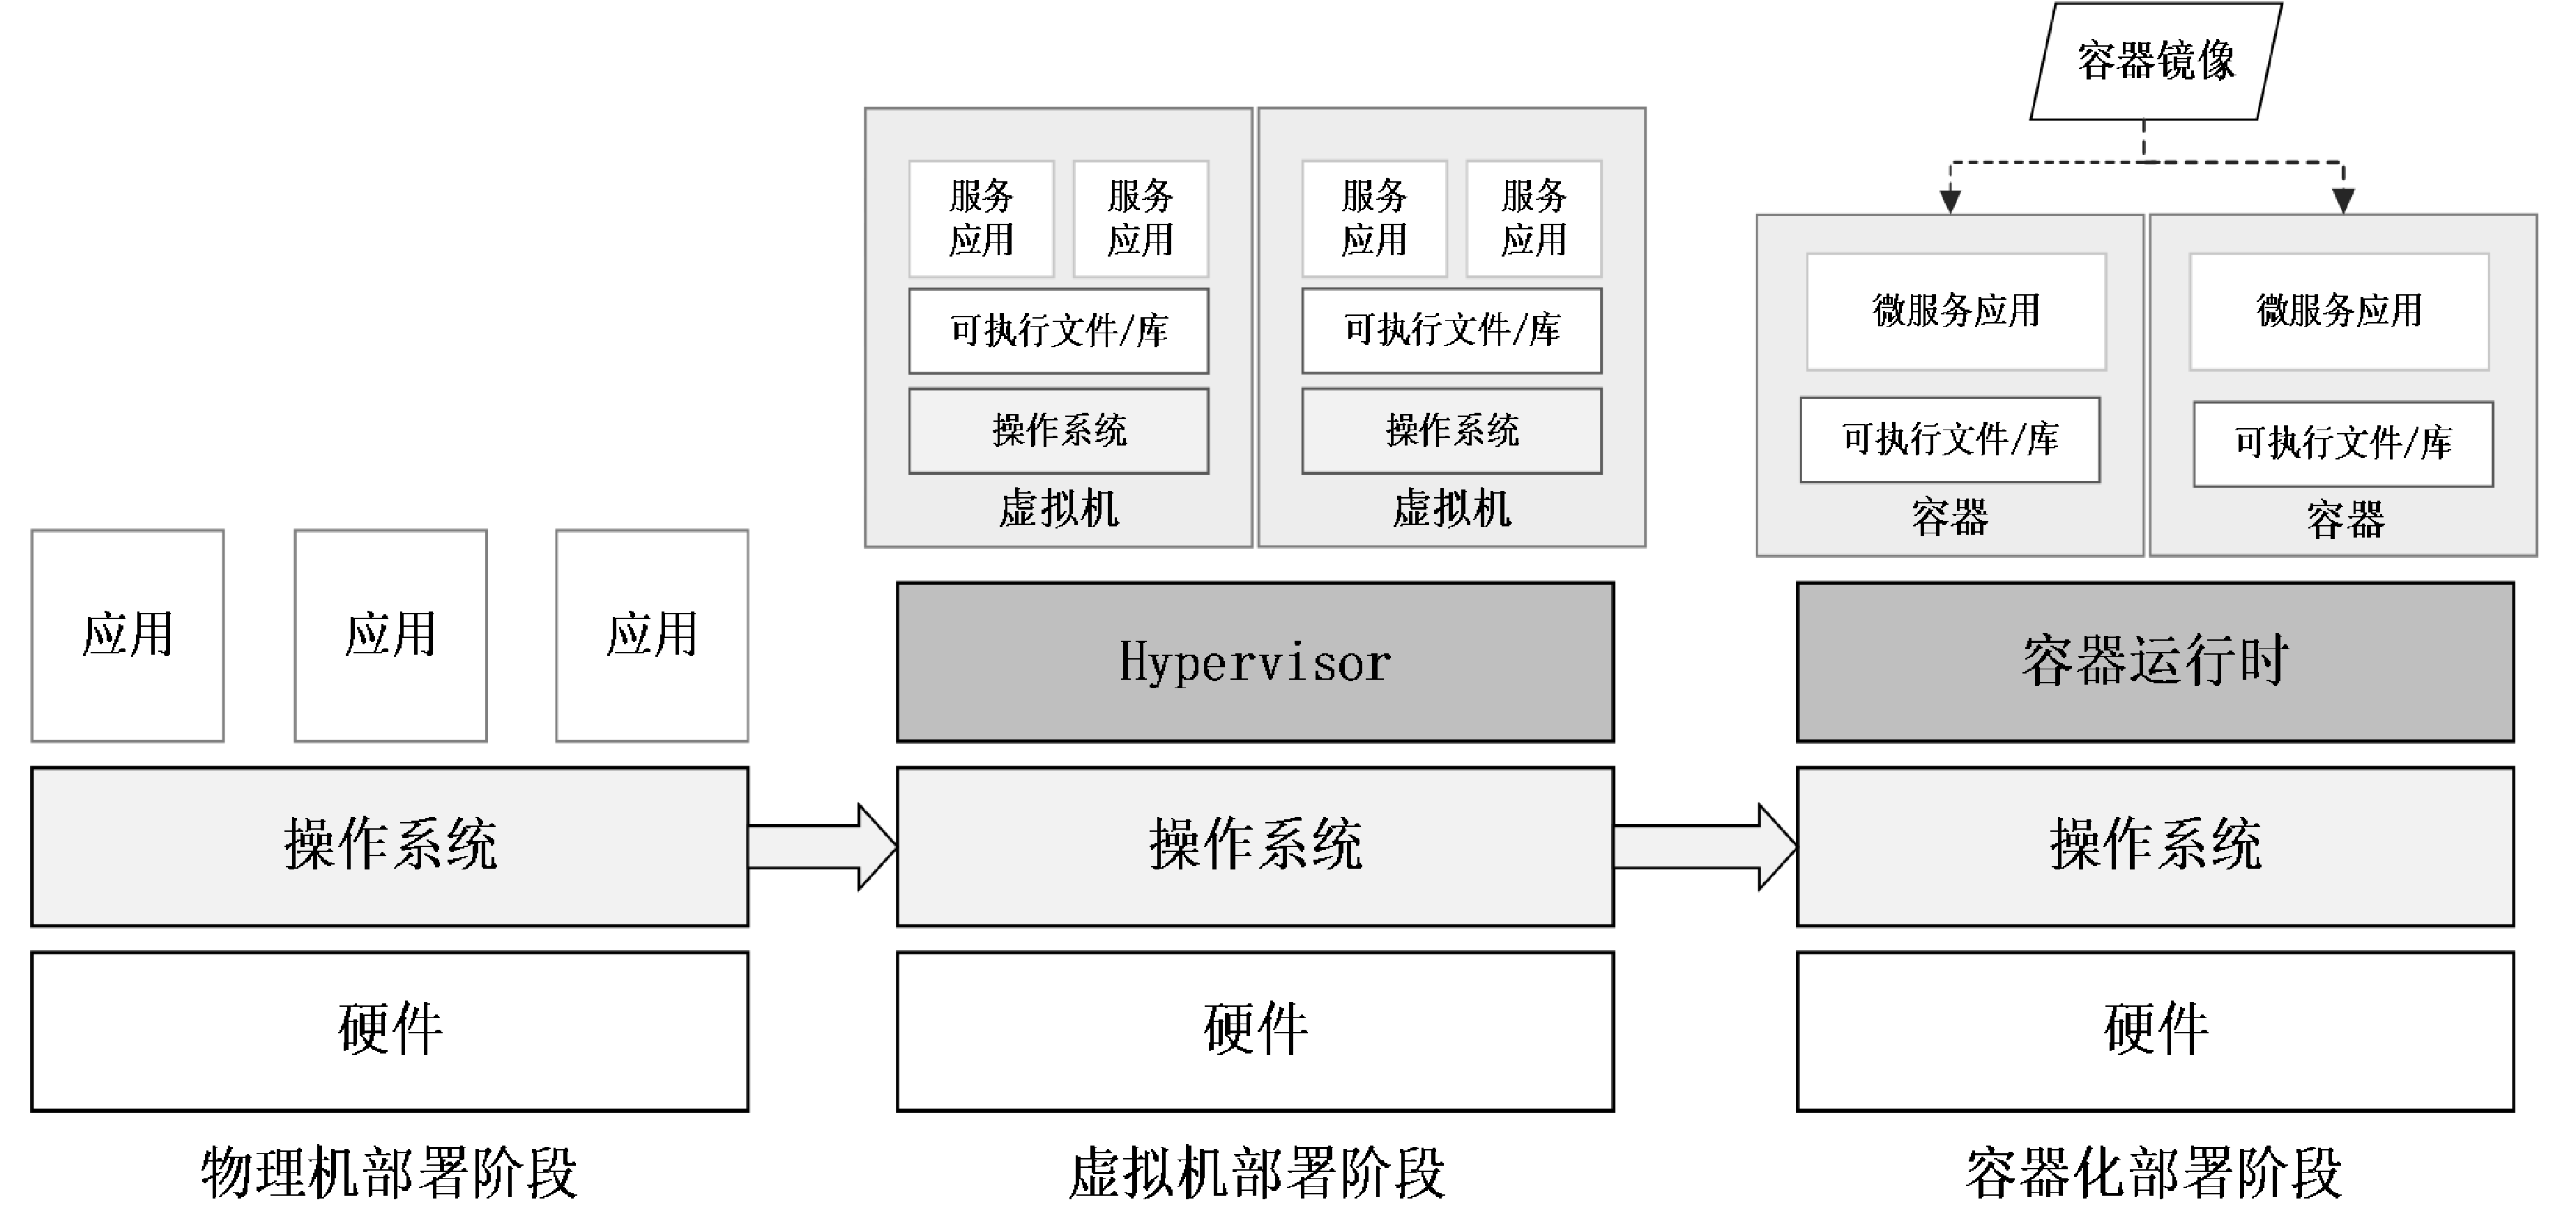
\includegraphics[width=0.9\linewidth]{images/容器.png}
    \bicaption{服务部署形式演进}{Evolution of service deployment paradigms}\label{fig:container-evolution}
\end{figure}

\begin{itemize}
    \item \textbf{命名空间（Namespace）隔离}：通过隔离进程、网络、挂载点等，使容器内运行的程序有独立系统抽象资源；
    \item \textbf{控制组（Cgroup）限制}：负责对容器施加 CPU、内存等硬件资源使用的强制规划，提供物理资源隔离；
    \item \textbf{只读分层与隔离挂载}：利用 OverlayFS 等联合文件系统\cite{wright2006versatility}，通过复用底层只读镜像并叠加独立的顶层读写区域，实现容器文件系统隔离。
\end{itemize}


\subsection{容器集群系统Kubernetes}
Kubernetes 是面向容器群集负载的分布式编排系统，简称K8S。源自于谷歌内部的虚拟化编排系统Borg\cite{Verma_2015}并在2014年正式对外开源。其核心思想是以\textbf{声明式 API}描述期望状态，再由控制平面持续驱动集群内容器向期望状态收敛\cite{kubernetes2024}。
\begin{figure}[htb]
    \centering
    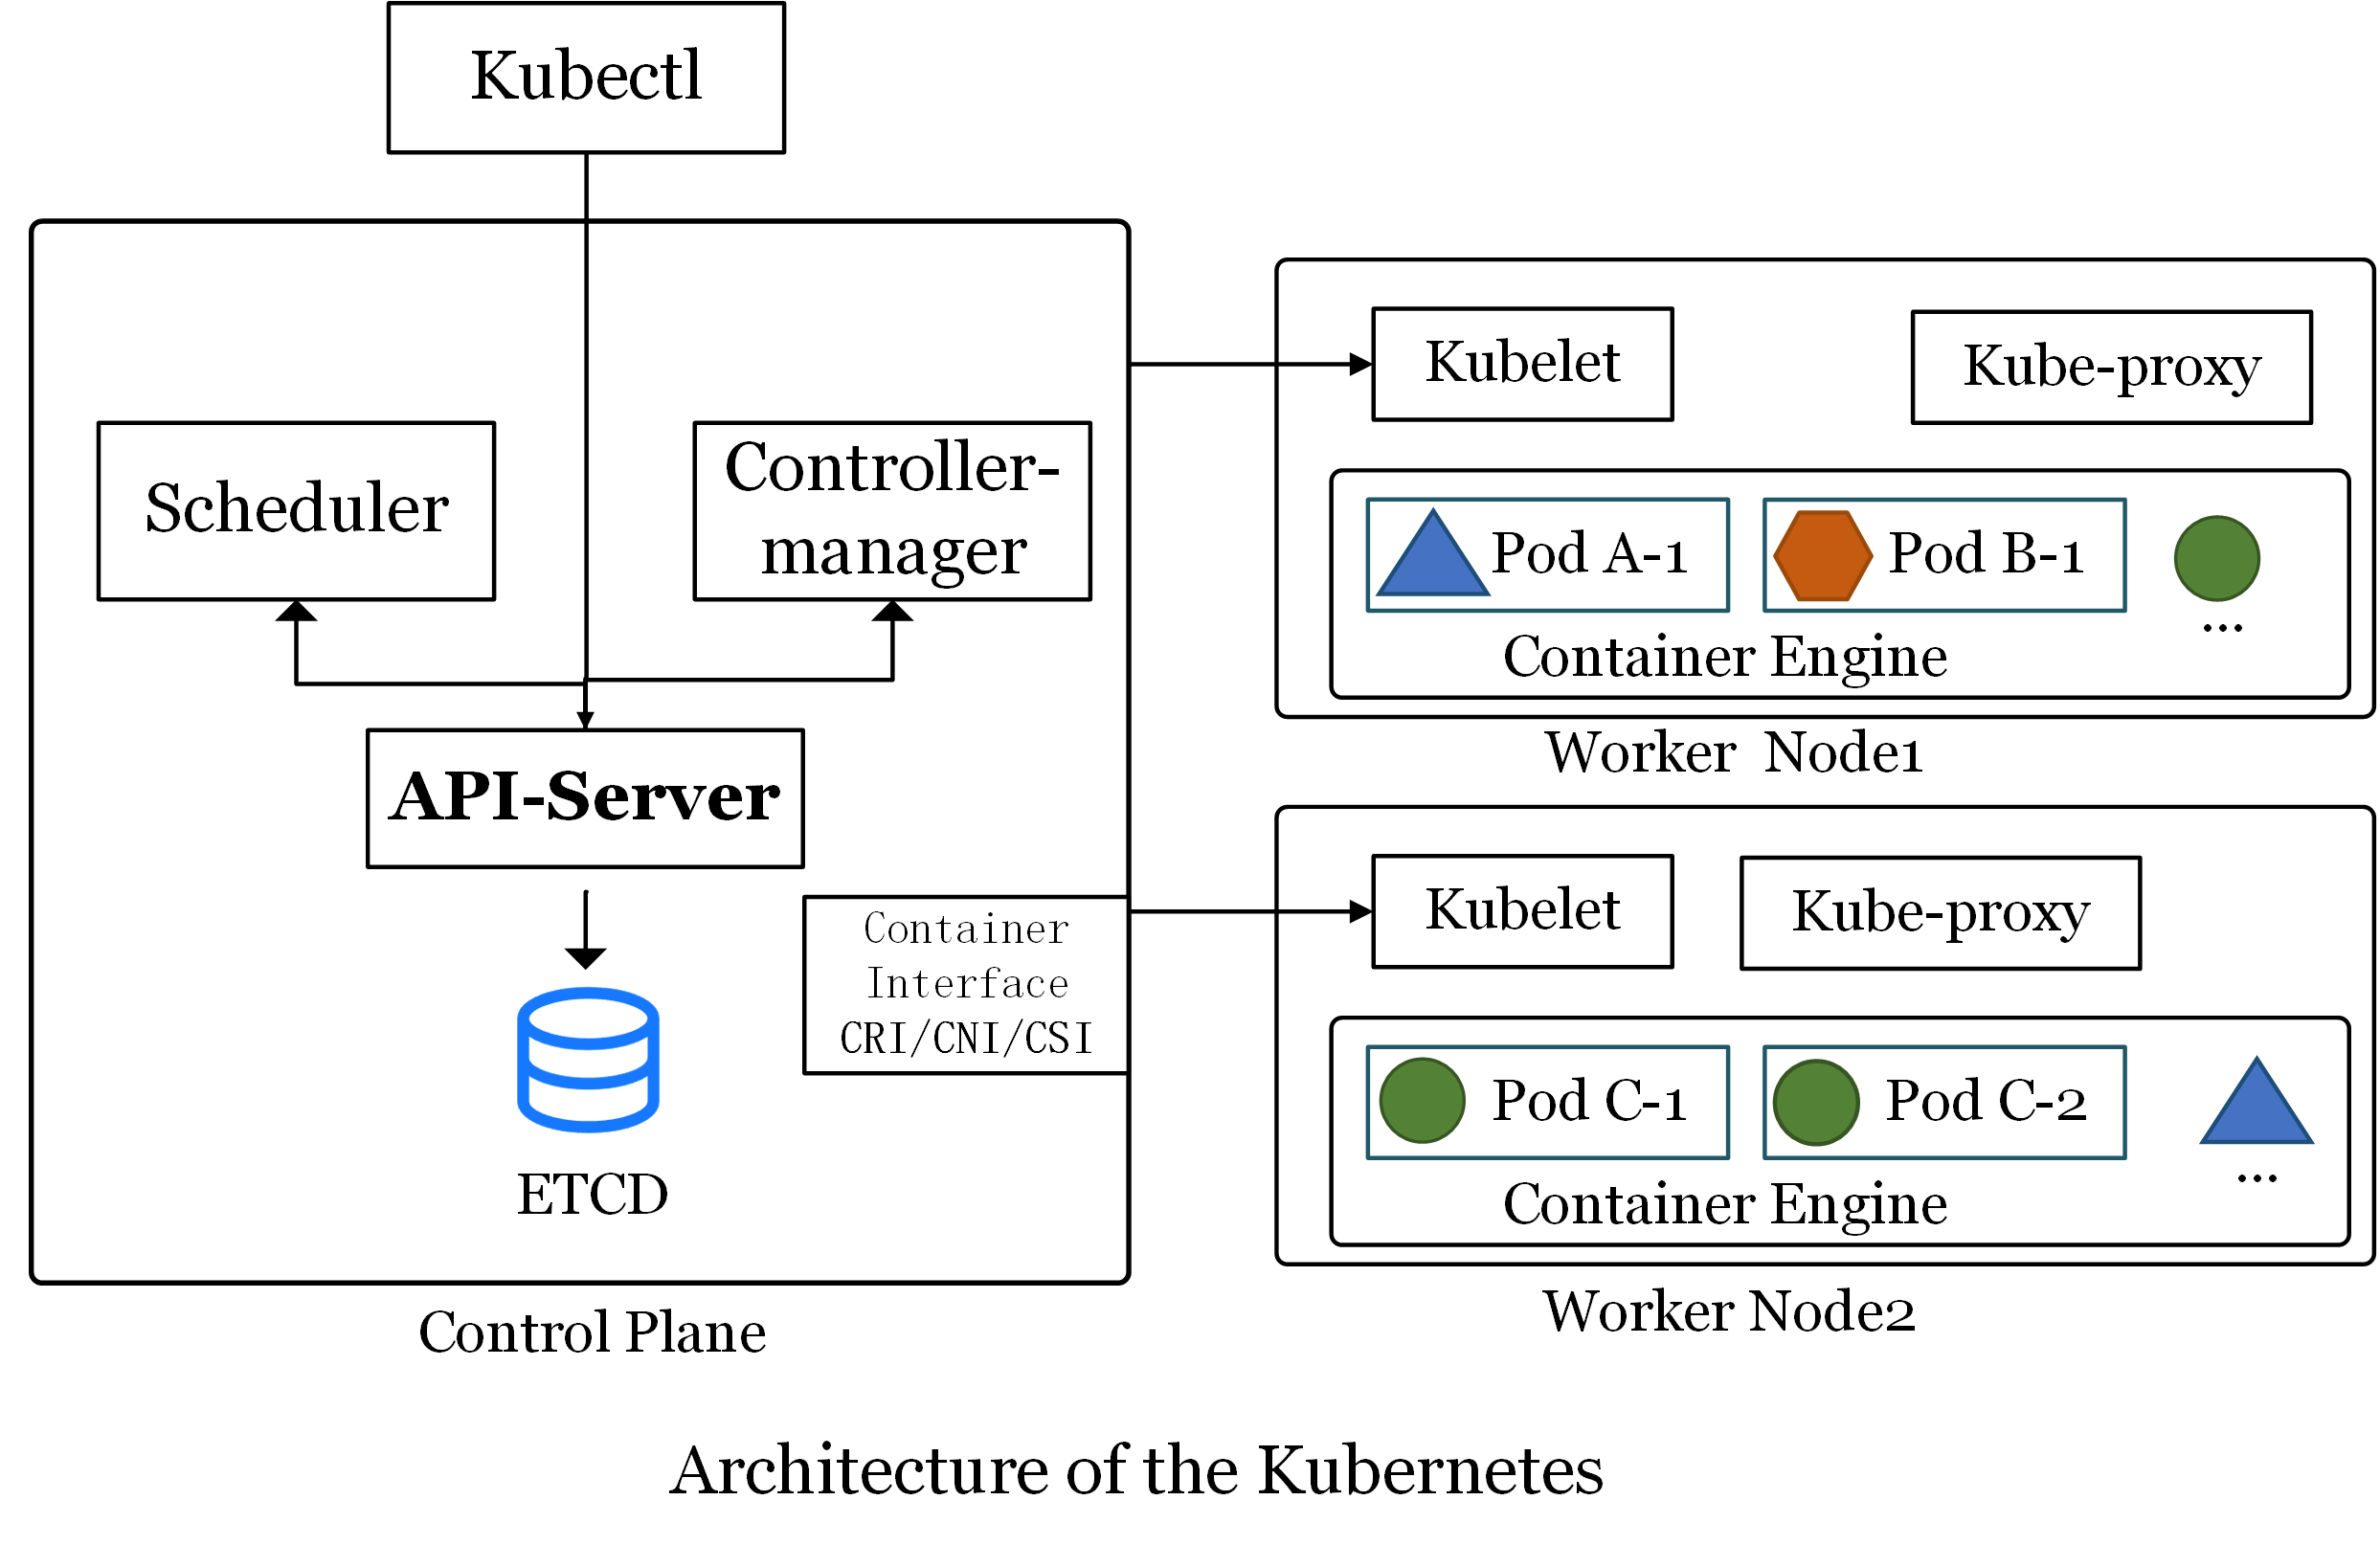
\includegraphics[width=0.8\textwidth]{images/k8s.png}
    \bicaption{Kubernetes 体系结构示意}{Overview of Kubernetes architecture}\label{fig:k8s-arch}
\end{figure}
图\ref{fig:k8s-arch}为 Kubernetes 的体系结构示意图，一个 Kubernetes 集群由\textbf{控制平面}与多个\textbf{工作节点}构成。控制平面负责提供控制接口、调度与集群控制逻辑，其中：\textbf{API Server}是所有资源访问与状态变更的统一入口，基于键值数据库ETCD承担认证、授权、准入与资源对象持久化等关键职责；\textbf{调度器}根据资源请求、亲和/反亲和等约束为工作负载选择节点；\textbf{控制器}负责提供控制与调节不同资源。工作节点侧，\textbf{kubelet}负责与API Server通信并维护调度到本节点的容器运行，\textbf{容器运行时}负责拉取镜像、创建容器并管理生命周期，\textbf{kube-proxy}负责服务转发与网络规则的实现。

Kubernetes通过一系列持久化\textbf{资源对象}表示集群对多种资源的编排与管理。例如，\textbf{Pod}是最小调度单元，包含一个或多个共享网络与存储的容器；Deployment/StatefulSet/DaemonSet分别面向无状态、有状态与节点守护型工作负载提供期望副本与更新策略；Service与Endpoint/EndpointSlice提供稳定的服务发现与负载均衡抽象；Ingress面向南北向流量提供入口控制；ConfigMap/Secret用于配置与敏感信息的声明式注入；Volume/PV/PVC则提供存储生命周期与绑定关系的抽象。


\subsection{Kubernetes 权限模型}
基于角色的访问控制（$\mathrm{RBAC}$）是 $\mathrm{Kubernetes}$ 授权机制的核心\cite{kubernetes2024}。图~\ref{fig:k8s-rbac-yaml}左侧展示了权限元模型的形式化表达，该权限模型可概括为\textbf{主语、动作与对象}的对应关系，即界定何种实体被允许对何种目标资源执行特定操作，其中：
\begin{itemize}
    \item \textbf{服务账户（ServiceAccount）}对应模型中的主语节点，代表发起请求的身份载体。在Kubernetes工作负载中每个Pod都有自己的服务账户。
    \item \textbf{权限角色（Role/ClusterRole）}对应模型中的动作与对象约束。该组件声明了在特定作用域内，针对各类资源（$\mathrm{resources}$）所允许执行的操作动词（$\mathrm{verbs}$）集合。
    \item \textbf{角色绑定（RoleBinding/ClusterRoleBinding）}作为关联映射机制，将服务账户与权限角色绑定以完成授权。
\end{itemize}

图~\ref{fig:k8s-rbac-yaml} 右侧展示了一个典型的 $\mathrm{RBAC}$ 授权流程示例：首先创建一个名为 $\mathrm{kada}$ 的 $\mathrm{ServiceAccount}$；随后定义名为 \texttt{basic-operation} 的 $\mathrm{Role}$，在其 $\mathrm{rules}$ 字段中授予对 $\mathrm{pods}$ 与 $\mathrm{secrets}$ 的 $\mathrm{get}$、$\mathrm{list}$、$\mathrm{create}$ 权限；最后通过 $\mathrm{RoleBinding}$ 将该 $\mathrm{Role}$ 绑定至 $\mathrm{kada}$ 账户。这种配置在接入第三方应用时很常见，但如果防范不当配置了过大的权限，将引发权限提升漏洞的风险。
\begin{figure}[htb]
    \centering
    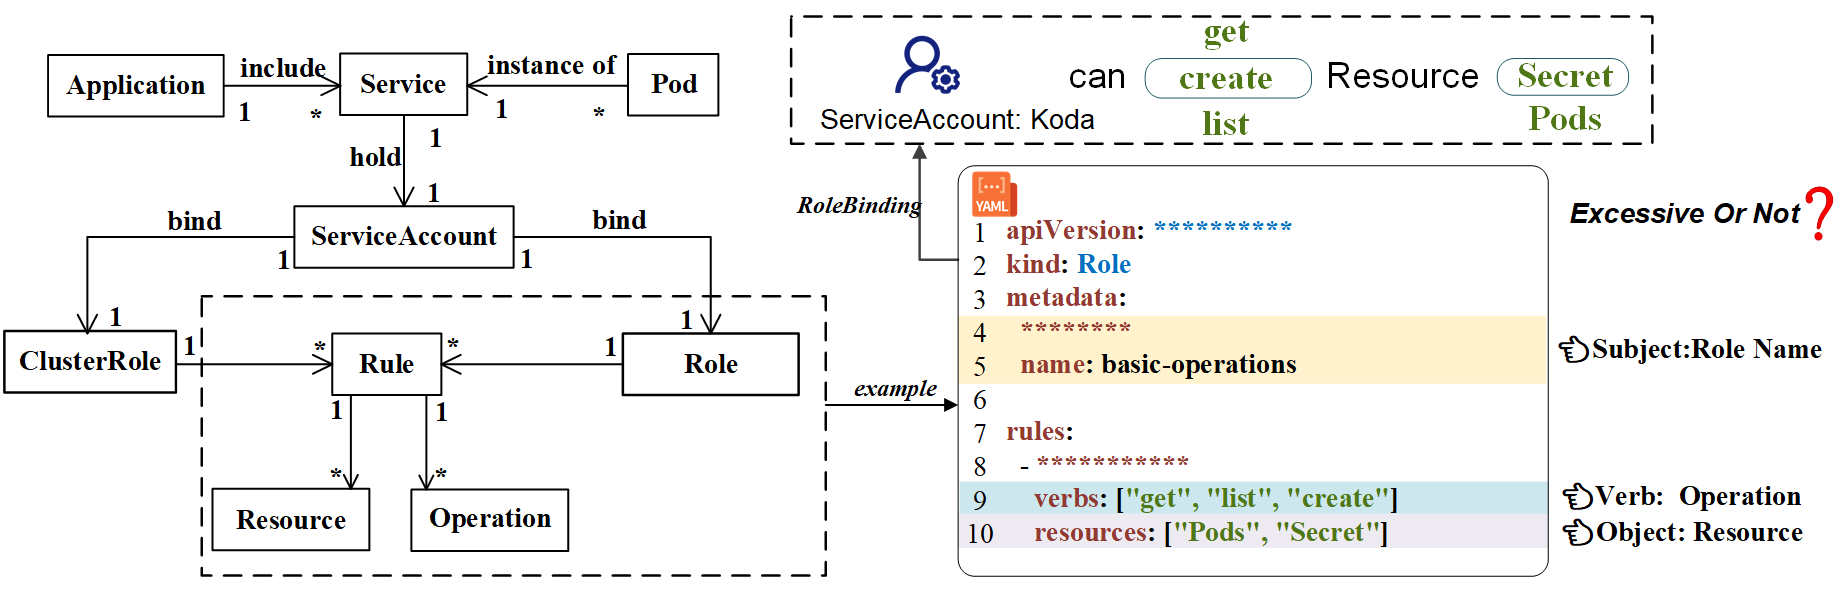
\includegraphics[width=0.95\textwidth]{images/yaml.png}
    \bicaption{Kubernetes RBAC 权限配置YAML文件示意\cite{kubeguard_icws2025}}{Example of Kubernetes RBAC permission configuration in YAML\cite{kubeguard_icws2025}}\label{fig:k8s-rbac-yaml}
\end{figure}

\subsection{Kubernetes 权限提升漏洞}

权限提升指攻击者在仅具备受限权限或初始执行能力的情况下，借助漏洞或错误配置，将自身权限提升到更高等级的过程\cite{mead2003computer}。在 Kubernetes 场景下，权限提升既可能表现为授权范围的扩大或横向获取，也可能表现为节点侧系统权限提升，从而对更大范围的资源与工作负载产生影响。

在云原生环境中，权限提升的危害往往具有更强的放大效应。一方面，单个节点通常承载多个 Pod，节点侧权限提升成功后，攻击者可能对同节点上的多个工作负载实施窃取敏感信息、篡改运行环境或注入恶意组件等行为。另一方面，Kubernetes 的资源对象与运维动作高度集中且自动化，控制平面授权不当同样会放大攻击后果。结合图~\ref{fig:k8s-rbac-yaml}中的示例，若主体被授予针对 $\texttt{Secret}$ 的 $\mathrm{get}/\mathrm{list}$ 权限，攻击者即可读取服务账户令牌、数据库口令或 API 密钥等敏感信息；若被授予针对 $\texttt{Pod}$ 的 $\mathrm{create}$ 权限，则可能进一步创建携带恶意镜像、特权配置或宿主机挂载的工作负载，作为横向移动、凭据窃取乃至后续节点侧利用的跳板。

图\ref{fig:cve-2024-33522} 以 \texttt{CVE-2024-33522} 为例展示了典型的节点侧权限提升漏洞。该漏洞源于 Calico CNI 安装程序的 SUID 位配置不当。若攻击者借助弱口令或服务暴露等前置手段获取了节点的本地访问权限，便可注入恶意二进制文件，并诱导安装程序以高权限执行。越权成功后，攻击者能直接接管容器运行时数据、窃取各类高优凭据并干扰网络组件，其危害将突破单一工作负载的隔离边界，迅速蔓延至整个集群。

\begin{figure}[htb]
    \centering
    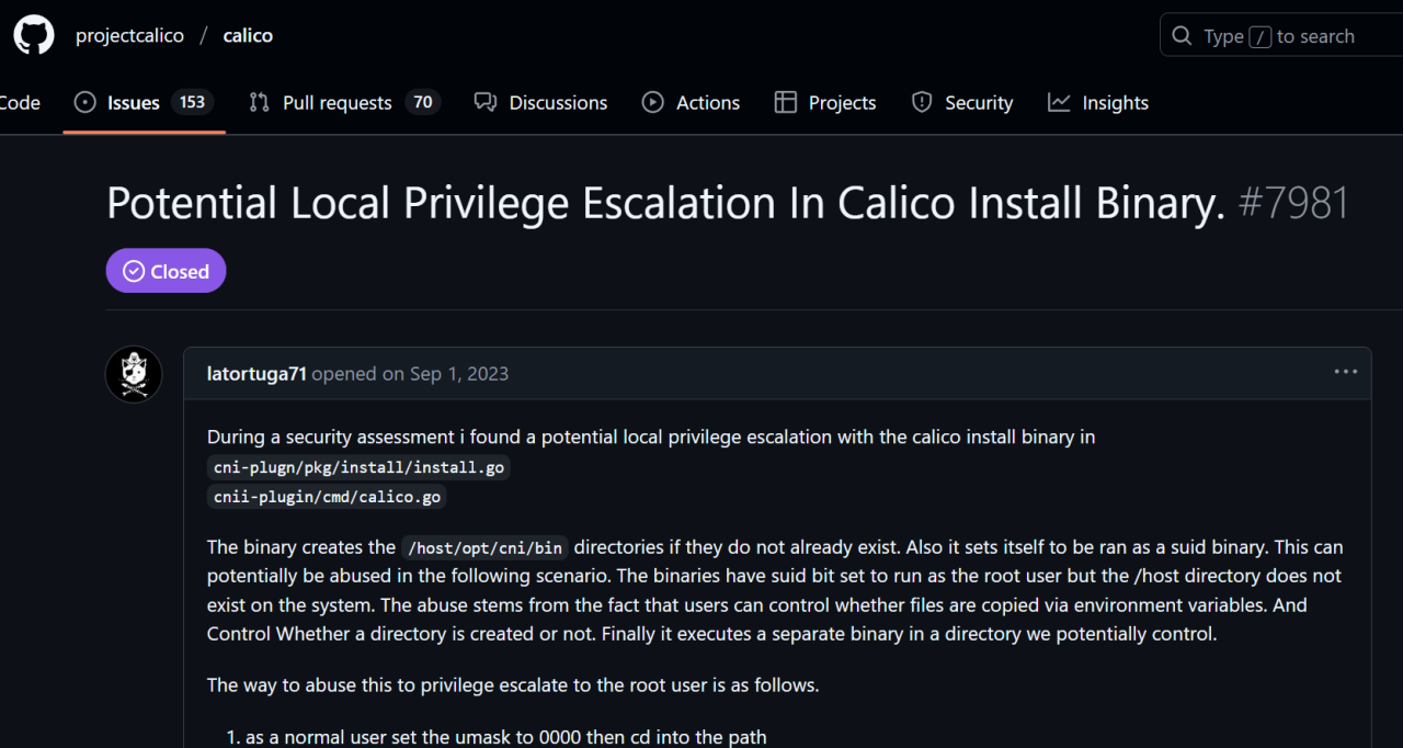
\includegraphics[width=1\textwidth]{images/cve_example.png}
    \bicaption{\texttt{CVE-\allowbreak2024-\allowbreak33522}（Calico）节点侧权限提升漏洞报告ISSUE}{Issue report of node-side privilege escalation vulnerability \texttt{CVE-\allowbreak2024-\allowbreak33522} in Calico}\label{fig:cve-2024-33522}
\end{figure}


\section{云原生安全工具}

云原生安全工具为 Kubernetes 集群提供全生命周期的安全风险监管机制。相关安全工具可基于规则化DSL代码对容器镜像、静态配置、集群系统行为、容器运行时等维度进行安全检查。下文将介绍几种广泛使用的云原生安全工具。

\subsection{监控工具：Falco}
Falco\cite{falco2025} 是云原生环境下广泛使用的开源容器运行时威胁检测引擎，其主要作用是为集群工作负载提供实时的异常行为监控与告警能力。在实现原理上，Falco 的机制包含内核态数据采集与规则引擎分析两个核心维度：它利用 eBPF 技术\cite{hoiland2018express}在内核层以极低侵入性的方式动态捕获各类系统调用事件，并将其转换为富含云原生上下文的事件流，随后交由基于领域特定语言构建的声明式规则引擎进行模式匹配，从而在不阻断正常业务的前提下识别并捕获风险行为。Falco同时也支持K8s业务监控，如K8s事件、K8s资源对象、K8s API调用等。

例如图\ref{fig:falco}展示了用于监测容器内启动交互式 shell 进程的规则。这种白盒化的检测方式具备极强的可解释性，能将告警直接关联至云原生实体，缩短安全定位路径。但该机制也存在一定的局限性：一方面，静态规则高度依赖专家知识的持续更新，对未知与变种攻击的泛化能力较弱；另一方面，其观测视野主要局限于系统调用层，难以有效感知应用层协议滥用或纯内存型的攻击。
\begin{figure}[htb]
    \centering
    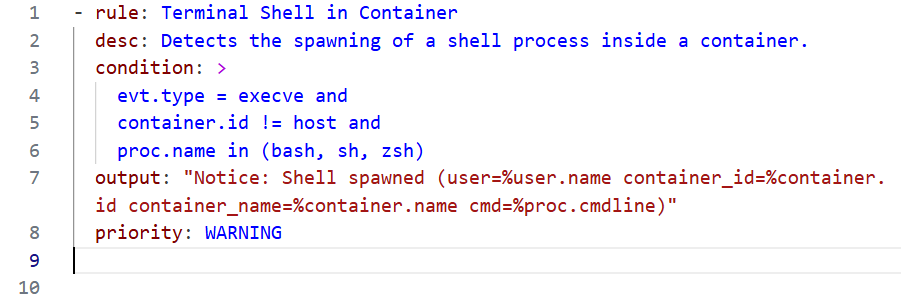
\includegraphics[width=0.8\textwidth]{images/falco.png}
    \bicaption{Falco 运行时监控与规则示意}{Illustration of Falco runtime monitoring and rules}\label{fig:falco}
\end{figure}

\subsection{防护工具：准入控制工具}
准入控制是 Kubernetes 中典型的事前防护机制。在 API Server 将资源持久化之前执行规则化校验，拦截特权容器、危险挂载、敏感权限增加等高风险配置变更。主流方案中，OPA/Gatekeeper 依托 Rego 语言，适合表达复杂组织策略；Kyverno 则采用 YAML 描述规则，更贴近运维习惯，落地成本更低。在补丁窗口期，这种规则化准入控制能够快速阻拦漏洞相关敏感资源操作。如图~\ref{fig:kyverno-demo} 所示，该Kyverno策略可以拒绝未携带 owner 标签的 Pod 创建请求。
\begin{figure}[htb]
    \centering
    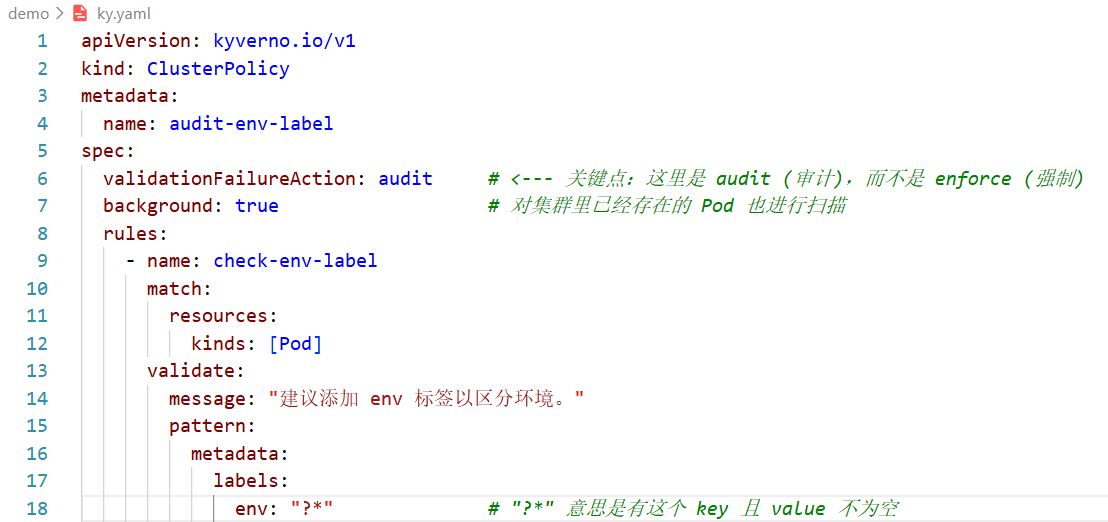
\includegraphics[width=0.8\linewidth]{images/kyverno.png}
    \bicaption{Kyverno 策略示例：强制要求 Pod 包含 owner 标签}{Example of a Kyverno policy enforcing owner labels on Pods}\label{fig:kyverno-demo}
\end{figure}

\subsection{网络防护工具：NetworkPolicy}
网络隔离用于降低横向移动与数据外传风险，是云原生环境中与身份权限控制互补的关键手段。Kubernetes 的 NetworkPolicy 为声明式防护策略，在多租户或微服务体系中可将控制域落到命名空间与工作负载级别，减少单点被攻破后对整个集群的扩散影响。常见的Kubernetes网络插件（如 Calico、Cilium、Weave Net 等）均支持 NetworkPolicy 的实现。
\begin{figure}[htb]
    \centering
    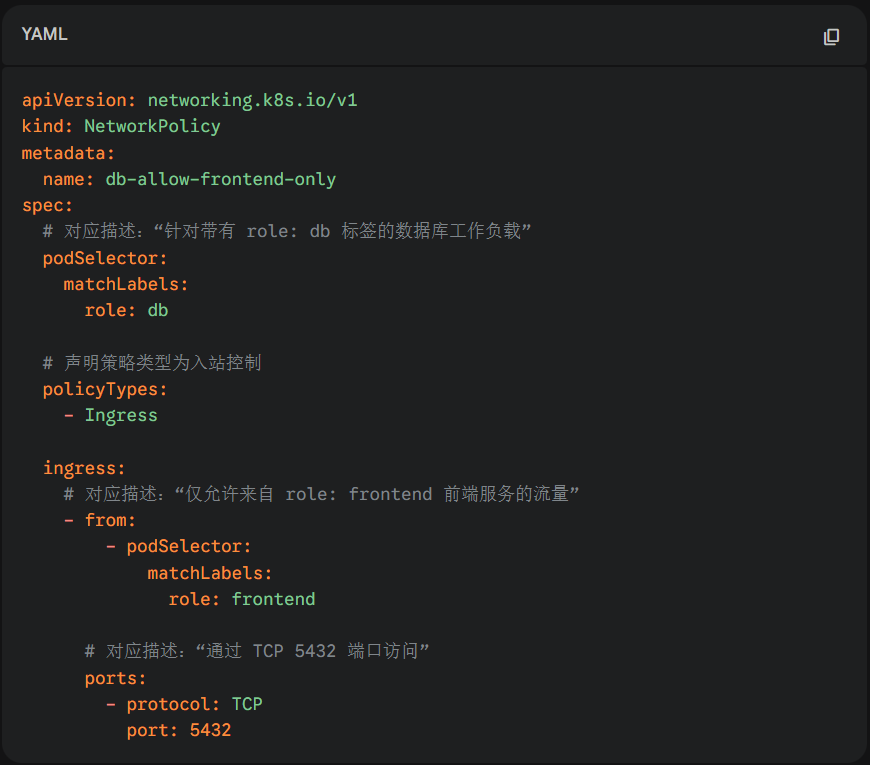
\includegraphics[width=0.8\linewidth]{images/networkpolicy.png}
    \bicaption{NetworkPolicy 示例：限制数据库仅允许前端服务访问}{Example of a NetworkPolicy allowing only frontend services to access the database}\label{fig:networkpolicy-demo}
\end{figure}

如图~\ref{fig:networkpolicy-demo} 所示，该策略定义了一个典型的微服务网络隔离场景：针对带有 \texttt{role: db} 标签的数据库工作负载，仅允许来自 \texttt{role: frontend} 前端服务的流量通过 TCP 5432 端口访问。这种基于标签选择器（Label Selector）的白名单机制有效地构建了微服务隔离边界，确保即使集群内其他容器试图横向移动访问数据库，也会在网络层被直接阻断。

\subsection{静态扫描与配置审计工具}
与运行时检测相对，静态扫描更偏向事前发现与持续治理。静态扫描在镜像构建、交付与部署前，通过自动化检查提前识别已知漏洞、弱配置与合规风险，避免高风险对象进入集群。

第一类是\textbf{镜像与依赖漏洞扫描}。该类工具通常解析镜像分层文件系统与软件包清单，基于公开漏洞库对已知 CVE 进行匹配，并输出风险等级、受影响版本与修复建议。代表性工具包括 Trivy\cite{trivy2025}、Grype/Anchore\cite{grype2025} 等；其中，Syft\cite{syft2025} 等工具可生成软件物料清单（SBOM），用于提升漏洞告警的可追溯性与供应链治理能力。

第二类是\textbf{Kubernetes 清单与基础设施即代码（IaC）扫描}。这类工具面向 YAML、Helm、Terraform 等配置，以规则化方式识别特权容器、宿主机路径挂载、过宽权限、明文密钥及资源限制缺失等风险，可用于代码评审、部署前基线核查与准入前置门禁。典型工具包括面向工作负载清单的 kube-linter\cite{kubelinter2025}、Kubescape\cite{kubescape2025}、kube-score\cite{kubescore2025}、KubeSec\cite{kubesec2025}、Polaris\cite{polaris2025}，以及面向 IaC 模板的 Checkov\cite{checkov2025}；针对权限审计的工具包括 KubiScan\cite{kubiscan2024}、Krane\cite{krane2024}、RBAC Police\cite{paloalto2024}。此类方法易于规模化落地，但也可能因业务差异产生误报，因此需要进行人工二次审查。表\ref{tab:k8s-security-scan-tools}对 Kubernetes 常见安全扫描与审计工具进行分类整理。
\begin{table}[htb!]
    \centering\bicaption{Kubernetes 常见安全扫描与审计工具整理}{Classification of common Kubernetes security scanning and auditing tools}\label{tab:k8s-security-scan-tools}
    \noindent\renewcommand{\arraystretch}{1.25}
    \setlength{\tabcolsep}{1.5mm}
    \small
    \begin{tabular}{>{\centering\arraybackslash}m{2.2cm}m{5.5cm}>{\raggedright\arraybackslash}m{4.0cm}}
    \toprule
    \textbf{类别} & \textbf{代表性工具} & \textbf{主要用途}\\
    \midrule
    镜像/依赖漏洞扫描
    & \texttt{Trivy}、\texttt{Grype}、\texttt{Clair}、\texttt{Snyk}
    & 发现镜像与依赖漏洞，用于 CI 门禁、制品准入与修复建议。\\
    \midrule
    SBOM 生成与供应链
    & \texttt{Syft}、\texttt{CycloneDX}、\texttt{cosign}
    & 生成 SBOM 与签名校验，用于供应链追溯和完整性校验。\\
    \midrule
    配置与 IaC 安全扫描
    & \texttt{Kubescape}、\texttt{kube-score}、\texttt{kube-linter}、\texttt{Polaris}、\texttt{KubeSec}、\texttt{datree}、\texttt{Checkov}、\texttt{KICS}、\texttt{tfsec}
    & 扫描 YAML/Helm/IaC 弱配置与基线违规，用于评审和部署前核查。\\
    \midrule
    RBAC/权限审计
    & \texttt{KubiScan}、\texttt{Krane}、\texttt{RBAC Police}、\texttt{kubeaudit}、\texttt{rakkess}、\texttt{kubectl-who-can}
    & 审计角色、绑定和账户权限，用于过宽授权识别与权限查询。\\
    \bottomrule
    \end{tabular}
\end{table}


\section{国内外研究现状}

本节按照通用系统权限安全研究、Kubernetes 场景安全研究和课题组已有工作这一顺序展开。前两部分分别概括权限提升风险在一般系统与云原生环境中的研究脉络，最后结合课题组前期成果说明本文工作的承接关系与问题切入点。

\subsection{系统权限安全问题}
系统权限安全研究最初聚焦访问控制模型与最小授权原则，随后逐步扩展到对过度授权、运行时提权行为和信息流泄露的综合治理。在基础设计原则层面，Saltzer 与 Schroeder\cite{saltzer1975protection}于 1975 年指出，\textbf{最小权限原则}是实现特权隔离的重要基础。基于这一原则，Ferraiolo 等\cite{ferraiolo1995role}提出基于角色的访问控制模型（RBAC），以角色组织多类权限并将其映射至不同主体，缓解了规模化授权中的管理难题。然而，\textbf{过度授权}现象普遍存在，显著扩大了系统攻击面\cite{o1995redundant}。为收敛这类风险，Molloy 等\cite{molloy2012generative}以及 Sanders 与 Yue\cite{sanders2018minimizing}分别提出基于日志与算法模型逆向生成应用最小权限集的策略，使权限治理由静态制度设计进一步走向结合实际使用行为的最小权限推断。

随着系统组件化程度不断提高，权限提升风险不再局限于单一主体的越权访问，而更多表现为跨组件、跨应用甚至跨平台的调用链滥用。在典型移动操作系统 Android 中，访问控制的粗粒度特性带来了更为突出的权限提升与隐蔽滥用风险。Davi 等人\cite{davi2010privilege}较早揭示了\textbf{混淆代理}攻击模型，即低权限应用可通过伪造合法请求，诱导高权限组件执行敏感操作。Hutchinson 等\cite{hutchinson2018survey}进一步将该模型概括为三个条件：请求敏感权限、开放导出组件以及存在通向敏感 API 的执行路径。随着攻防对抗持续升级，提权漏洞的利用方式也由单一组件劫持\cite{wu2016seccomp}，演变为多重调用链上的跨应用共谋\cite{elzawawy2025hidden}，甚至扩展至同一设备内由第三方 SDK 发起的共谋攻击\cite{taylor2017intralibrary}。

围绕上述风险，现有治理方法大致可归纳为静态架构分析、动态行为监控和数据流追踪三类。静态方法中，Au 等\cite{au2012pscout}提出 PScout，通过分析系统源码自动提取底层权限检查图谱；后续研究进一步结合最小执行权限要求引入强制访问控制机制：Bagheri 等\cite{bagheri2019deldroid}提出 DelDroid，通过静态分析自动推导并强制实施应用所需的最小权限架构；Wu 等\cite{wu2016seccomp}提出 SecComp，在组件调用层面约束非授权操作以防御劫持攻击。动态方法中，相关研究结合进程代数建模\cite{xu2019adaptive}、系统级探针监控\cite{hussain2020framework}以及深度学习与半监督学习\cite{sharmeen2020adaptive}，实现运行期权限提升行为的拦截与预警。当授权边界被突破后，还可借助数据流监控开展后果溯源，相关研究已从面向 Web 的混合污点分析\cite{tripp2009taj}，拓展至 Android 系统层实时信息流监控（TaintDroid\cite{enck2014taintdroid}）和免 Root 的动态污点分析（TaintMan\cite{you2017taintman}）。整体来看，这一路径表明权限安全分析正由权限静态归属分析进一步转向对真实调用链利用过程的分析。

上述思路随后被扩展到小程序等宿主内嵌生态的权限安全研究。Zhang 等\cite{zhang2023small}对多个主流小程序生态开展系统性研究，提取了通用的权限控制抽象模型，揭示了跨运行态环境下的多类典型越权漏洞并通过实际攻击加以验证；Wang 等\cite{wang2024minichecker}则聚焦小程序数据权限滥用问题，定义了多种违规权限申请模式，并设计静态分析工具 MiniChecker 开展规模化检测，指出现有平台权限机制在底层设计上仍存在固有缺陷。总体来看，通用系统中的相关研究为识别跨组件调用、越权传播和后果溯源提供了重要方法基础，但其分析对象和执行环境与 Kubernetes 仍存在明显差异。

\subsection{Kubernetes 安全问题}
在云原生场景中，Kubernetes 将配置、控制平面、网络与运行时机制耦合在同一系统之中，权限风险往往沿部署模板、授权链路和组件交互同时扩散。因此，相关研究既继承了通用系统中的最小授权与行为检测思路，又形成了更强调配置语义和多层联动的分析路径。现有工作大体可分为配置风险识别、模板与 IaC 安全分析、架构与权限链风险挖掘以及网络与运行时防护四类。

安全误配置是 Kubernetes 场景中最常见、也最早受到关注的风险来源。早期研究主要用于勾勒配置风险的整体图景：Islam Shamim 等\cite{Islam_Shamim_2020}系统总结了 Kubernetes 安全实践，Shamim\cite{Shamim_2021}进一步指出部署清单偏离最佳实践可能直接演化为可利用的提权路径，Curtis 与 Eisty\cite{Curtis_2025}基于 Stack Overflow 数据的实证分析也表明配置安全始终是开发侧的核心关切。在此基础上，Rahman 等\cite{k8smanifests2023}对开源清单中的典型安全误配置进行了大规模归纳与实证研究。然而，仅依赖静态扫描难以完整反映风险的真实可利用性。Shamim 等\cite{shamim2025prescription}评估了 CIS 推荐配置的合规现状，发现从业人员对安全基线的理解存在显著差异，现有 SAST 工具的检测覆盖也有明显不足；其后续工作\cite{shamim2025dastk8s}进一步结合工业界部署实践，论证了将 DAST 动态分析纳入配置核验流程的客观必要性。上述研究说明，Kubernetes 配置安全研究正由基线合规判断转向实际可利用风险评估。

在识别单份清单风险之外，基础设施即代码（IaC）也被证明是 Kubernetes 安全风险的重要来源。针对 Helm Charts 带来的依赖传播与供应链风险，Zerouali 等\cite{Zerouali_2023}和 Blaise 与 Rebecchi\cite{Blaise_2022}分别从生态规模与依存关系角度提供了分析基础；Minna 等\cite{minna2025analyzing}进一步评估了大语言模型在修复 IaC 配置异味方面的效果与边界。为缓解多平台安全语义碎片化问题，Ul Haque 等\cite{KGSecConfig2022}提出知识图谱框架 KGSecConfig，对安全配置概念进行统一抽取与建模。这类研究表明，Kubernetes 安全治理已由局部规则检查逐步扩展到面向模板、依赖关系与安全语义的自动化分析。

仅分析配置项是否合规仍不足以解释攻击链如何形成，因此相关研究进一步深入到体系结构缺陷与过度授权所引发的链式风险。Dell'Immagine 等\cite{Dell_Immagine_2023}面向微服务部署定义了一组安全反模式，并实现自动检测工具 KubeHound，表明安全缺陷可能嵌入系统交互结构之中。Yang 等\cite{yang2023take}系统分析了 CNCF 生态中第三方插件的权限配置，设计了多种攻击路径利用策略，可将工作节点逃逸演化为全集群接管。Gu 等\cite{gu2024epscan}提出 EPScan，通过面向容器的程序分析自动比对实际资源访问行为与声明权限，识别可被利用的过度特权。与前述误配置研究相比，这一方向更关注风险沿授权链路的形成与放大机制。

即便控制平面配置与授权链路得到一定约束，底层网络与运行时隔离仍是 Kubernetes 安全防护不可缺少的一环。容器编排引入的网络抽象与传统安全模型存在显著差异，Minna 等\cite{Minna_2021}指出这种差异可能衍生非预期的攻击路径。在网络策略的工程落地层面，Budigiri 等\cite{Budigiri_2021}基于 eBPF 评估了网络策略的性能代价，Kim 等\cite{Kim_2025}对比了多种容器网络接口插件的安全能力，两项工作共同揭示了协议过滤深度与转发性能之间的固有权衡。在缓解机制方面，研究视角涵盖了从 DevOps 流水线到节点侧运行时的多个层面：Pecka 等\cite{pecka2022privilege}通过构造流水线攻击场景证明了工具合规并不等同于安全，Cesarano 与 Natella\cite{cesarano2025kubefence}提出的 KubeFence 通过裁剪非必要 API 参数实现了比 RBAC 更细粒度的接口过滤，Zhu 与 Gehrmann\cite{Zhu_2022}和 Le 等\cite{Le_2023}则分别在 AppArmor 配置自动生成与系统调用感知调度方向上强化了节点侧防护。综合来看，现有研究已经从清单级合规检查推进到跨组件授权链与运行时隔离的综合分析，但对于权限提升漏洞在暴露窗口期如何快速生成兼顾监控与防护的协同策略，仍缺乏统一方法框架。


\subsection{本课题组研究基础}
在上述研究基础上，课题组围绕 Kubernetes 权限风险检测开展了系统研究，已形成覆盖风险建模、原型实现与实验验证的前期积累。其中，代表性成果为 KubeGuard 框架。该框架面向过度权限、权限提升和敏感信息泄露三类风险，分别设计了最小权限集构建、规则化审计以及敏感词监测机制\cite{kubeguard_icws2025}。如图\ref{fig:kgf}所示，KubeGuard 由过度权限检测、权限提升检测和敏感信息泄露检测三个模块构成。

\begin{figure}[htb]
    \centering
    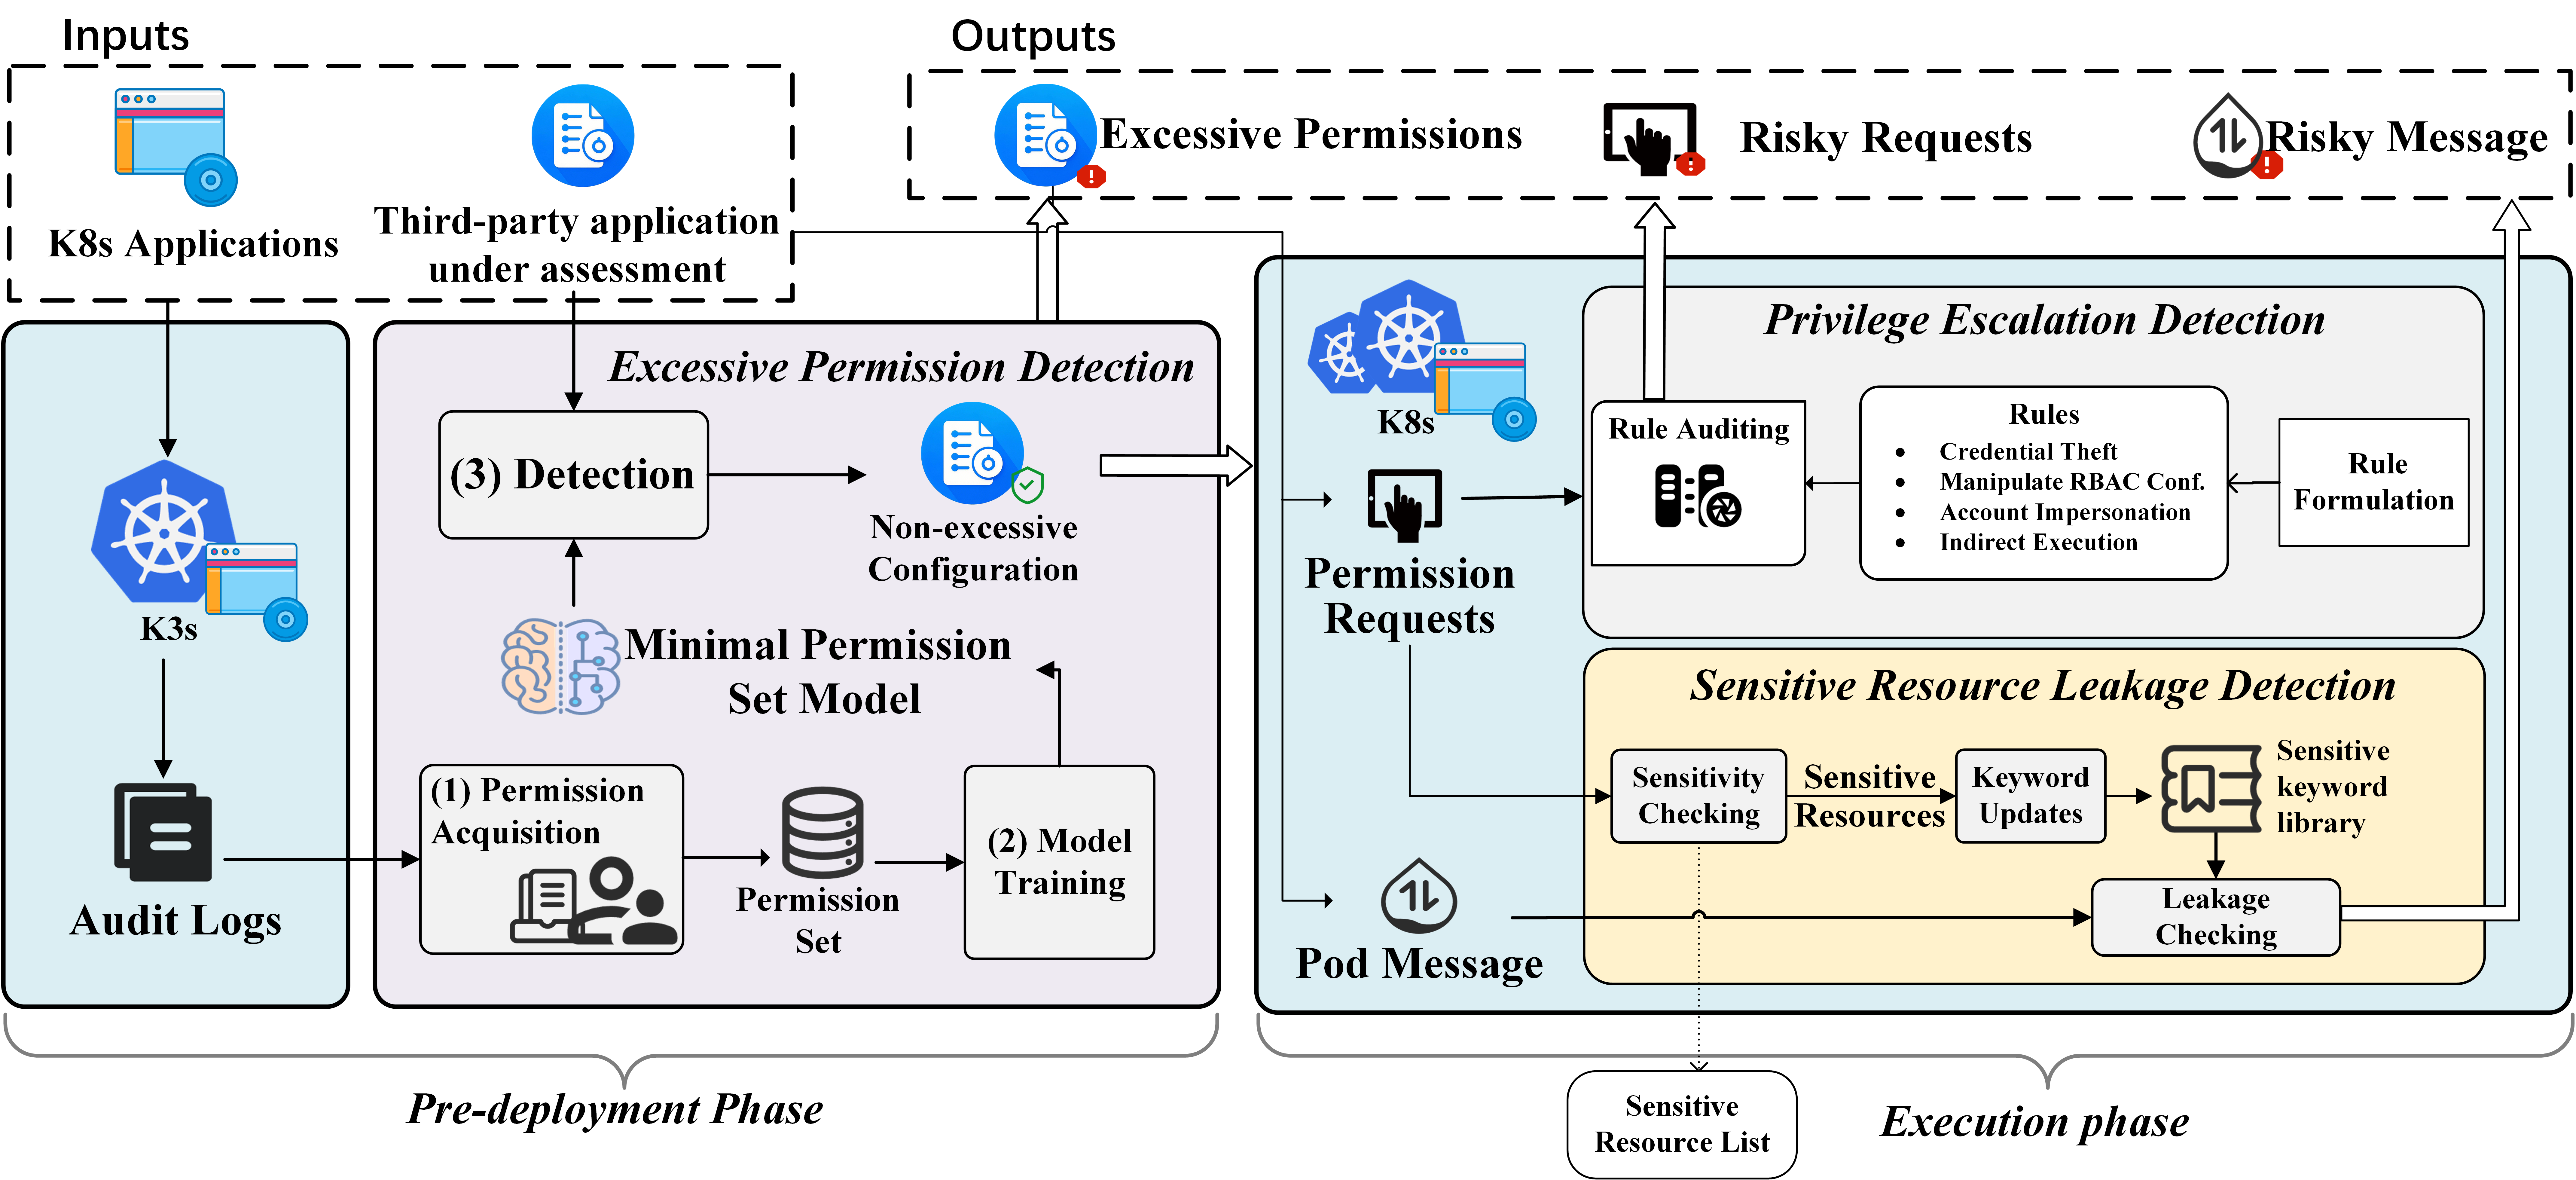
\includegraphics[width=0.95\textwidth]{images/KGF.png}
    \bicaption{KubeGuard 方法框架图\cite{kubeguard_icws2025}}{Framework of the KubeGuard method\cite{kubeguard_icws2025}}\label{fig:kgf}
\end{figure}

在方法设计上，KubeGuard 一方面利用 NLP 技术识别应用所需的最小权限集，以判定权限配置是否存在过度授权；另一方面通过动态规则审计检测多类权限提升风险。具体而言，该工作将权限提升场景归纳为凭证窃取、账户冒用、RBAC 操纵和间接执行四类，并针对各类场景提出相应的检测思路。考虑到规则细节较为繁杂，相关风险描述与检测规则在正文中不再展开，具体内容见附录表\ref{tab:PEDetectionRules}。此外，该框架还通过监测 Pod 间消息传输并结合关键词匹配，对涉及敏感资源的内容进行告警，从而覆盖敏感信息泄露风险。

在系统实现与效果验证方面，课题组进一步实现了原型系统 KubeGuarder，并在开源 Kubernetes 应用与模拟场景中开展实验评估\cite{kubeguard_icws2025}。实验结果表明，该系统在过度权限检测方面相较静态基线方法表现出更高的有效性与准确性，同时能够识别多类型的权限提升与敏感信息泄露风险。这说明前期工作已经验证了从权限视角开展风险建模与检测的可行性，并为本文进一步研究提供了方法与系统基础。

不过，现有工作仍主要停留在权限层面的规则化检测，其核心依据是 RBAC 配置与 API 访问行为之间的匹配关系。该方法虽然能够较为系统地覆盖多种权限提升模式，但在真实生产环境中仍存在三方面局限：（1）仅依据权限配置与操作行为的对应关系，难以准确区分正常运维行为与恶意提权行为，因此误报风险较高；（2）该方法主要面向控制平面与资源访问层，尚未深入节点侧系统层面的权限提升漏洞，对容器逃逸、SUID 配置不当及内核漏洞等底层利用缺乏针对性的检测能力；（3）基于预定义规则的检测方式对未知漏洞与新型攻击手法的泛化能力有限。上述不足也构成了本文进一步研究的直接出发点，即在保留权限视角优势的同时，引入面向真实利用链与运行态场景的检测与防护能力。


\section{小结}
本章介绍了容器、Kubernetes 及其权限模型等基础概念与云原生安全工具，并从系统权限安全、Kubernetes 安全与课题组前期工作三个层面梳理了国内外研究现状，为后续章节的方法设计与实验验证奠定了理论基础。
